%To generate pdf:
%pdflatex description.tex

\documentclass{article}

\usepackage[letterpaper, margin=0.5in, footskip=4ex]{geometry}
\usepackage{xcolor}
\usepackage{graphicx} % Required to insert images
\usepackage{float} % For placing figures EXACTLY where I say
\usepackage{epstopdf}
\usepackage{listings} % Required for insertion of code
%%\usepackage{enumitem}
\usepackage{amssymb,amsmath}
%%\usepackage[open, openlevel=2]{bookmark}
\usepackage[hidelinks=true,bookmarks=true,bookmarksopen=true]{hyperref}

\usepackage[backend=biber, style=chem-biochem, sorting=anyt]{biblatex}
\addbibresource{parts/refs.bib}

\graphicspath{ {fig_pdf/} } %If additional directories are needed, place them in additional sets of inner braces e.g {fig_pdf/}{fig_svg/}

\setlength{\parindent}{0pt}
\setlength{\parskip}{1ex}

\begin{document}

\title{Problem Description for Diffusion Through Nanopore}
\author{Tom Pace}
\maketitle

\tableofcontents

%===============================================================================
\section{Background}\label{sec:background}

We study a silica membrane containing nanoscopic circular pores arranged in a two-dimensional lattice.
We desire to understand the rate of transport of different ions through the nanopores,
quantified in terms of an effective diffusion constant.
The pore geometry is variable, as is the diffusion equation governing transport.
The diffusion equation is solved using \texttt{FEniCS}.

%===============================================================================
%not a stand-alone document; intended for inclusion in a larger document

\section{Geometry and Finite Element Mesh}\label{sec:geometry-and-mesh}

%-------------------------------------------------------------------------------
\subsection{System Geometry}\label{subsec:geometry}

We study both a body-centered rectangular lattice of pores,
as well as a face-centered lattice of pores.
The unit cell geometry has two planes of symmetry.
This symmetry is used to reduce the model to only one quarter of the unit cell.

The body-centered geometry is shown in Figure \ref{fig:body-intro}.
The face-centered geometry is shown in Figure \ref{fig:face-intro}.

\begin{figure}[H]
\centering
\includegraphics[width=1\textwidth]{body-intro.pdf}
\caption{Body-centered geometry}
\label{fig:body-intro}
\end{figure}

\begin{figure}[H]
\centering
\includegraphics[width=1\textwidth]{face-intro.pdf}
\caption{Face-centered geometry}
\label{fig:face-intro}
\end{figure}

The geometric variables are:

$\begin{array}{rcl}
Sx & = & 2 Lx =\text{Unit cell x-dimension} \\
Sy & = & 2 Ly =\text{Unit cell y-dimension} \\
Lx & = & \frac{Sx}{2} =\text{Model x-dimension} \\
Ly & = & \frac{Sy}{2} =\text{Model y-dimension} \\
R & = & \text{Pore radius} \\
tm & = & \text{Membrane thickness} = \text{Pore length} \\
H & = & \text{Distance from membrane surface to model boundary}
\end{array}$


%-------------------------------------------------------------------------------
\subsection{Mesh Generation}\label{subsec:meshgen}

\texttt{gmsh} is used to generate the finite element mesh.
The mesh is generated from solid geometry defined by its boundary surfaces.
These surfaces, in turn, are defined by their boundaries,
which are defined using points.

\textcolor{red}{\textbf{TODO}}: gmsh geometry (point numbers, etc)


%===============================================================================
%not a stand-alone document; intended for inclusion in a larger document

\section{Definitions}

%-------------------------------------------------------------------------------
\subsection{System of Units}\label{subsec:units}

\texttt{FEniCS} does not generally keep track of the units used in either its inputs or its outputs.
Accordingly, a consistent set of units must be provided for all inputs,
and also used to interpret all outputs.
This is done by selecting a minimal set of fundamental units,
and then deriving the units of all other quantities in terms
these fundamental units.

The fundamental dimensions and units selected for this problem are:
\begin{description}
  \item [Length:] nanometers (nm)
  \item [Amount of substance:] number of particles (particles)
  \item [Time:] nanoseconds (ns)
  \item [Energy:] electron-Volts (eV)
  \item [Temperature:] Kelvin (K)
  \item [Electric charge:] fundamental charge (e)
\end{description}

From the fundamental units and dimensions, the following are derived:
\begin{description}
  \item [Concentration:] particles per cubic nanometer (particles/nm\textsuperscript{3})
  \item [Particle Flux (vector field):] particles per nanometer squared per nanosecond (particles/nm\textsuperscript{2}/ns)
  \item [Integrated Particle Flux (scalar quantity):] particles per nanosecond (particles/ns)
  \item [Electric Potential:] Volts (V)
\end{description}

The implicit units above can be converted to other units with the following conversion factors:
\begin{description}
  \item [Molarity (M):]
  $\frac{1 \,\mathrm{particle}}{\mathrm{nm}^3} = \frac{1 \,\mathrm{particle}}{\mathrm{nm}^3}
  \frac{1 \,\mathrm{mole}}{6.022 \cdot 10^{23} \,\mathrm{particles}} \left(\frac{10^9 \,\mathrm{nm}}{\mathrm{m}}\right)^3 
  \frac{(10^{-1}\,\mathrm{m})^3}{1 \,\mathrm{L}}
  = 1.661 \,\frac{\mathrm{moles}}{\mathrm{L}}$
  \item [millimoles/liter (mM):] $\frac{1 \,\mathrm{particle}}{\mathrm{nm}^3} = 1,661 \,\frac{10^{-3}\,\mathrm{moles}}{\mathrm{L}}$
\end{description}

\textcolor{red}{\textbf{TODO}}: provide conversion factors for the other direction as well (from model units to common ones)

%-------------------------------------------------------------------------------
\subsection{Effective Diffusion Constant}\label{subsec:D_eff}

To compute the effective diffusion constant,
the three-dimensional diffusion problem is considered from the perspective of a simpler one-dimensional diffusion problem.
Specifically, we wish to consider diffusion in the direction across the membrane.
The Fickian diffusion equation (see Section \ref{sec:unhom_fick}) in one dimension can be written as

\begin{equation}\label{eq:fickslaw_1D}
j = - D_{\mathrm{bulk}} \frac{\mathrm{d}c}{\mathrm{d}s}
\end{equation}

where:

$\begin{array}{rcl}
s & = & \text{position within the one-dimensional domain} \\
j & = & j(s) = \text{flux at any point, in units of number of particles per unit area per unit time} \\
D_{\text{bulk}} & = & \text{diffusion constant of the medium, in units of area per unit time} \\
c & = & c(s) = \text{concentration at any point, in units of number of particles per unit volume} \\
\frac{\mathrm{d}c}{\mathrm{d}s} & = & \text{first spatial derivative of concentration}
\end{array}$

The three-dimensional problem is converted to an equivalent one-dimensional problem
by integrating over the area of the unit cell, in the two directions perpendicular to
the one-dimensional diffusion problem.
The total flux across the membrane will be given by:

\begin{equation}
J_{\mathrm{cell}} = - D_{\mathrm{bulk}}\int_{\mathrm{cell}} \mathrm{d}A\, \frac{\partial c}{\partial s}
\end{equation}

We define the effective diffusion constant such that the integrated flux is the same,
when used with an the average concentration gradient across the membrane:

\begin{equation}\label{eq:Deff_Jcell}
J_{\mathrm{cell}} = - D_{\mathrm{eff}} A_{\mathrm{cell}} \frac{\Delta c}{\Delta s}
\end{equation}

where:

$\begin{array}{rcl}
J_{\text{cell}} & = & \text{integral of flux over the pore, in units of number of particles per unit time} \\
A_{\text{cell}} & = & \text{area of unit cell} \\
D_{\text{eff}} & = & \text{unknown effective diffusion constant} \\
\Delta c & = & \text{change in concentration} \\
\Delta s & = & \text{distance over which concentration changes}
\end{array}$

Re-arranging this equation to solve for the unknown $D_{\mathrm{eff}}$, we have:

\begin{equation}\label{eq:Deff_def}
D_{\mathrm{eff}} = - \frac{J_{\mathrm{cell}}}{A_{\mathrm{cell}}} \frac{\Delta s}{\Delta c}
\end{equation}

The integrated flux, $J_{\mathrm{model}}$, is calculated from the model by integrating
the ion flux over a surface parallel to the membrane surface.
The result should be the same for any such surface capturing the full extents of the model.
That is, the integrated flux should be the same when integrating over the model pore as
when integrating over the upgradient or downgradient boundary of the model.

Specifically, the integrated flux is calculated as:

\begin{equation}
J_{\mathrm{model}} = \int_{\mathrm{model}} \mathrm{d}A\, \left(\hat{n} \cdot \vec{j} \right)
 = - D_{\mathrm{bulk}} \int_{\mathrm{model}} \mathrm{d}A\, \left(\hat{n} \cdot \vec{\nabla} c \right)
\end{equation}

where $\hat{n}$ is the directed normal to the surface,
and $c$ is the concentration field found by solving the model.

Because of the use of planes of symmetry (see Section \ref{subsec:silica_membrane}),
the flux obtained by integration is only one quarter of the total for the unit cell.
That is, $J_{\mathrm{cell}} = 4 J_{\mathrm{model}}$.
With $A_{\mathrm{cell}} = 4 Lx Ly$, we have:

\begin{equation}
D_{\mathrm{eff}} = - \frac{4 J_{\mathrm{model}}}{4 Lx Ly} \frac{\Delta s}{\Delta c}
 = - \frac{J_{\mathrm{model}}}{Lx Ly} \frac{\Delta s}{\Delta c}
\end{equation}

For convenience, we define the integral

\begin{equation}
I_{\mathrm{gc}} = \int_{\mathrm{model}} \mathrm{d}A\, \left(\hat{n} \cdot \vec{\nabla} c \right)
\end{equation}

then the flux integral is simply

\begin{equation}
J_{\mathrm{model}} = - D_{\mathrm{bulk}} I_\mathrm{gc}
\end{equation}

and the effective diffusion constant is

\begin{equation}
D_{\mathrm{eff}} = D_{\mathrm{bulk}} \frac{I_\mathrm{gc}}{Lx Ly} \frac{\Delta s}{\Delta c}
\end{equation}

This can also be written as

\begin{equation}
\frac{D_{\mathrm{eff}}}{D_{\mathrm{bulk}}} = \frac{I_\mathrm{gc}}{Lx Ly} \frac{\Delta s}{\Delta c}
\end{equation}

The values of $\Delta c$ and $\Delta s$ are calculated by extracting
the concentration result at two points located symmetrically on opposite sides of the membrane.
The difference in concentration between these two points is $\Delta c$,
and the distance between them is $\Delta s$.

Slightly different results for the value of $D_{\mathrm{eff}}$ could be attained by selecting different
pairs of symmetrically located points.
For consistency, the results here are taken with these two points located
along the centerline of the pore, at both faces of the membrane.

%-------------------------------------------------------------------------------
\subsection{Free Volume Fraction}\label{subsec:volfrac}

The free volume fraction, $\phi$ is defined here as

\begin{equation}
\phi = \frac{\text{pore area}}{\text{unit cell area}}
= \frac{\pi R^2}{Sx Sy} = \frac{\pi R^2}{4 Lx Ly}
\end{equation}


%===============================================================================
%not a stand-alone document; intended for inclusion in a larger document

\section{Unhomogenized Fickian Diffusion Equation}\label{sec:unhom_fick}

%-------------------------------------------------------------------------------
\subsection{Governing Differential Equation}\label{subsec:unhom_fick_gov}

\textcolor{red}{\textbf{TODO}}: need equation reference


For particle flux defined as 

\begin{equation}
  \vec{j} = - D_{\mathrm{bulk}} \vec{\nabla} c
\end{equation}

The Fickian diffusion equation can be written:
\begin{equation}
  \frac{\partial c}{\partial t} = - \vec{\nabla} \cdot \vec{j}
\end{equation}

where:

$\begin{array}{rcl}
c & = & c(x,y,z) = \text{the particle concentration field (number of particles per unit volume)} \\
t & = & \text{time} \\
\vec{j} & = & \vec{j}(x,y,z) = \text{the particle flux field (number of particles per unit area per unit time)} \\
D_{\mathrm{bulk}} & = & \text{the implicit diffusion constant of the solvent (unit area per unit time)}
\end{array}$

For constant $D_{\mathrm{bulk}}$, this can be written as

\begin{equation}
  \frac{\partial c}{\partial t} = D_{\mathrm{bulk}} \nabla^2 c
\end{equation}

We seek the steady-state solution, defined by
  $\frac{\partial c}{\partial t} = 0$ at all points in the problem domain.
Thus, we seek to solve

\begin{equation}
  D_{\mathrm{bulk}} \nabla^2 c = 0
\end{equation}

subject to boundary conditions.

Assuming $D_{\mathrm{bulk}}$ is any nonzero constant, this is clearly the same as

\begin{equation}
  \boxed{
    \nabla^2 c = 0
  }
\end{equation}


%-------------------------------------------------------------------------------
\subsection{Weak Form}\label{subsec:unhom_fick_weak}

For solution in \texttt{FEniCS}, a weak form of this equation is required.
Multiplying by a test function $v$ and integrating over the problem domain,

\begin{equation}
  \int_{\Omega} \left(\nabla^2 c \right) v \,\mathrm{d}^3x = 0
\end{equation}

Using the product rule
\begin{equation}
  \vec{\nabla} \cdot \left( v \vec{\nabla} c \right) =
  v \left(\vec{\nabla} \cdot \vec{\nabla} c \right) + \vec{\nabla}c \cdot \vec{\nabla}v =
  v \left(\nabla^2 c \right) + \vec{\nabla}c \cdot \vec{\nabla}v
\end{equation}

\begin{equation}\label{eq:product_rule_divergence}
  \left(\nabla^2 c \right) v =
  \vec{\nabla} \cdot \left( v \vec{\nabla} c \right) - \vec{\nabla}c \cdot \vec{\nabla}v
\end{equation}

to integrate by parts, the equation becomes
\begin{equation}
  \int_{\Omega} \left(\nabla^2 c \right) v \,\mathrm{d}^3x =
  \int_{\Omega} \vec{\nabla} \cdot \left( v \vec{\nabla} c \right) \,\mathrm{d}^3x
  - \int_{\Omega} \left( \vec{\nabla}c \cdot \vec{\nabla}v \right) \,\mathrm{d}^3x =0
\end{equation}

Applying the divergence theorem (Gauss's theorem):
\begin{equation}
  \int_{\partial\Omega} \left( \hat{n} \cdot \vec{\nabla} c \right) v\,\mathrm{d}s
  - \int_{\Omega} \left( \vec{\nabla}c \cdot \vec{\nabla}v \right) \,\mathrm{d}^3x = 0
\end{equation}

\begin{equation}
  \int_{\Omega} \left( \vec{\nabla}c \cdot \vec{\nabla}v \right) \,\mathrm{d}^3x =
  \int_{\partial\Omega} \left( \hat{n} \cdot \vec{\nabla} c \right) v\,\mathrm{d}s
\end{equation}

In this case, we have both Dirichlet and von Neumann boundary conditions:
there are some boundary surfaces where the concentration is known,
and others where the particle flux is known.
Specifically, known concentrations are applied at both the top and bottom of the model,
and the particle flux must be zero for all other boundary surfaces.
Defining $\Gamma_D$ as the Dirichlet boundary surfaces,
and $\Gamma_N$ as the von Neumann boundary surfaces, we obtain

\begin{equation}
  \int_{\Omega} \left( \vec{\nabla}c \cdot \vec{\nabla}v \right) \,\mathrm{d}^3x =
  \int_{\Gamma_D} \left( \hat{n} \cdot \vec{\nabla} c \right) v\,\mathrm{d}s
  +\int_{\Gamma_N} \left( \hat{n} \cdot \vec{\nabla} c \right) v\,\mathrm{d}s
\end{equation}

For the Dirichlet boundary surfaces (where the concentration is known),
the test function $v$ must be equal to zero,
as the variation of the unknown function must be zero at points where the function is known.

Furthermore, a flux of zero requires that the derivative of the concentration in a direction
normal to the boundary surface is zero.
That is, $\hat{n} \cdot \vec{\nabla} c = 0$ at all points on the von Neumann boundaries.

Therefore, the governing equation is simply
\begin{equation}
  \int_{\Omega} \left( \vec{\nabla}c \cdot \vec{\nabla}v \right) \,\mathrm{d}^3x = 0
\end{equation}

In terms of \texttt{FEniCS}, this means that the bilinear form is

\begin{equation}
  \boxed{
    a(c,v)=\left( \vec{\nabla}c \cdot \vec{\nabla}v \right) \,\mathrm{d}^3x
  }
\end{equation}

and the linear form is constant, zero, provided there are no nonzero Neumann boundary conditions.

%-------------------------------------------------------------------------------
\subsection{Expected Results}\label{subsec:unhom_fick_expected}

The effective diffusion constant of Section \ref{subsec:D_eff}
was derived by simplification of the governing equation
to an unhomogenized Fickian diffusion equation.
Consequently, the effective diffusion constant for this equation
can be estimated very simply.

In the absence of surface chemistry phenomena,
we should expect the concentration gradient
to be essentially constant within the pore, and oriented only in the axial direction.
That is, the concentration profile within the pore will be linear,
and at any cross-section there is only a single value of the concentration.
This implies that the problem is very nearly one-dimensional,
as assumed in the definition of $D_{\mathrm{eff}}$.

Defining the concentration gradient within the pore as
\begin{equation}
  \vec{\nabla} c = \left(\frac{\mathrm{d}c}{\mathrm{d}s}\right)_{\mathrm{pore}} \hat{n}
\end{equation}

where $\left(\frac{\mathrm{d}c}{\mathrm{d}s}\right)_{\mathrm{pore}}$ is a constant,
the integrated flux within the pore is

\begin{equation}
  J_\mathrm{cell} = -D_\mathrm{bulk} \int_\mathrm{cell} \mathrm{d}A\, \left(\frac{\mathrm{d}c}{\mathrm{d}s}\right)_{\mathrm{pore}}
  = -D_\mathrm{bulk} A_\mathrm{pore} \left(\frac{\mathrm{d}c}{\mathrm{d}s}\right)_{\mathrm{pore}}
\end{equation}

Note that the area in this formula is the area of the pore only,
rather than the entire unit cell, because only the pore is within the problem domain
at a cross-section through the pore.

From equation \ref{eq:Deff_Jcell}, we have

\begin{equation}
  J_{\mathrm{cell}} = - D_{\mathrm{eff}} A_{\mathrm{cell}} \frac{\Delta c}{\Delta s}
\end{equation}

But with a constant concentration gradient,

\begin{equation}
  \frac{\Delta c}{\Delta s} = \left(\frac{\mathrm{d}c}{\mathrm{d}s}\right)_{\mathrm{pore}}
\end{equation}

So,

\begin{equation}
  J_{\mathrm{cell}} = - D_{\mathrm{eff}} A_{\mathrm{cell}} \left(\frac{\mathrm{d}c}{\mathrm{d}s}\right)_{\mathrm{pore}}
  = -D_\mathrm{bulk} A_\mathrm{pore} \left(\frac{\mathrm{d}c}{\mathrm{d}s}\right)_{\mathrm{pore}}
\end{equation}

This simplifies to

\begin{equation}
  \frac{D_\mathrm{eff}}{D_\mathrm{bulk}} = \frac{A_\mathrm{pore}}{A_\mathrm{cell}}
\end{equation}

which matches the definition of the free volume fraction from Section \ref{subsec:volfrac}, so

\begin{equation}
  \boxed{
    \frac{D_\mathrm{eff}}{D_\mathrm{bulk}} = \phi
  }
\end{equation}

for unhomogenized Fickian diffusion.


%===============================================================================
%not a stand-alone document; intended for inclusion in a larger document

\subsection{Unhomogenized Smoluchowski Equation}\label{subsec:unhom_smol}

%-------------------------------------------------------------------------------
\subsubsection{Governing Differential Equation}\label{subsubsec:unhom_smol_gov}

\textcolor{red}{\textbf{TODO}}

%-------------------------------------------------------------------------------
\subsubsection{Weak Form}\label{subsubsec:unhom_smol_weak}

\textcolor{red}{\textbf{TODO}}

%-------------------------------------------------------------------------------
\subsubsection{Applied Potential}\label{subsubsec:unhom_smol_potential}

\textcolor{red}{\textbf{TODO}}

%-------------------------------------------------------------------------------
\subsubsection{Expected Results}\label{subsubsec:unhom_smol_expected}

The Smoluchowski diffusion equation does not model any interaction between the ions themselves.
Therefore, with an applied potential of zero,
the solution should be the same as for the
unhomogenized Fickian diffusion equation (Section \ref{subsubsec:unhom_fick_expected}).

\textcolor{red}{\textbf{TODO}}



%===============================================================================
%not a stand-alone document; intended for inclusion in a larger document

\section{Unhomogenized Poisson-Nernst-Planck Equation}\label{sec:unhom_pnp}

%-------------------------------------------------------------------------------
\subsection{Governing Differential Equations}\label{subsec:unhom_pnp_gov}


\textcolor{red}{\textbf{TODO}}: need reference for PNP equation

We consider $N_s$ ion species interacting through the an electrostatic potential.
The concentration field of each species is $c_s$, where $s=1 ... N_s$ is the index over the species.
The charge of each ion species is $z_s$, so that the volumetric charge density associated
with ion species $s$ is $z_s c_s$.
The overall volumetric charge density is therefore given by:

\begin{equation}
  \rho = \sum_{s=1}^{N_s}z_s c_s
\end{equation}

From the Poisson equation, the electric potential is therefore governed by:

\begin{equation}\label{eq:Poisson_for_ions}
  \boxed{
    -\epsilon_{0}\epsilon_{r} \nabla^2 \Phi = \sum_{s=1}^{N_s}z_s c_s
  }
\end{equation}

For each ionic species, the change in concentration over time is related to the ion flux as:

\begin{equation}
  \frac{\partial c_s}{\partial t} = - \nabla \cdot \vec{j}_s
\end{equation} 

with ion flux defined as:

\begin{equation}
  \vec{j}_s  = -D_s \left( \nabla c_s + \beta z_s c_s \nabla \Phi \right)
\end{equation}

The governing equation for each ion species is therefore:

\begin{equation}
  \frac{\partial c_s}{\partial t} = \nabla \cdot \left(
  D_s \left( \nabla c_s + \beta z_s c_s \nabla \Phi \right)
  \right)
\end{equation}

Under the assumption that the diffusion constant does not vary spatially,
this becomes:

\begin{equation}
  \frac{\partial c_s}{\partial t} = 
  D_s \left( \nabla^2 c_s + \beta z_s \nabla \cdot \left( c_s \nabla \Phi \right) \right)
\end{equation}

\begin{equation}\label{eq:PNP_timedep}
  \boxed{
    \frac{\partial c_s}{\partial t} = 
    D_s \left( \nabla^2 c_s + \beta z_s \left( \nabla c_s \cdot \nabla \Phi \right)  + \beta z_s c_s \nabla^2 \Phi \right)
  }
\end{equation}

The steady-state condition is therefore governed by

\begin{equation}\label{eq:PNP_steady_state_gov}
  \boxed{
    \nabla^2 c_s + \beta z_s \left( \nabla c_s \cdot \nabla \Phi \right)  + \beta z_s c_s \nabla^2 \Phi = 0
  }
\end{equation}


%-------------------------------------------------------------------------------
\subsection{Weak Form}\label{subsec:unhom_pnp_weak}

The weak form of the Poisson equation is derived by multiplying
Equation \ref{eq:Poisson_for_ions} by a test function $v_\phi$
associated with the electric potential,
and then integrating over the problem domain.

\begin{equation}
  -\epsilon_{0}\epsilon_{r} \int_\Omega \left( \nabla^2 \Phi \right) v_\phi \,\mathrm{d}^3x
   = \sum_{s=1}^{N_s} \int_\Omega z_s c_s v_\phi \,\mathrm{d}^3x
\end{equation}

Performing an integration by parts using the product rule
of Equation \ref{eq:product_rule_divergence}, this becomes

\begin{equation}
  -\epsilon_{0}\epsilon_{r}
  \left( \int_\Omega \nabla \cdot \left( v_\phi \nabla \Phi \right) \,\mathrm{d}^3x
  - \int_\Omega  \left( \nabla \Phi \cdot \nabla v_\phi \right) \,\mathrm{d}^3x \right)
  - \sum_{s=1}^{N_s} \int_\Omega z_s c_s v_\phi \,\mathrm{d}^3x = 0
\end{equation}

Applying the divergence theorem yields

\begin{equation}
  \boxed{
    -\epsilon_{0}\epsilon_{r} \int_{\partial\Omega} \left( \hat{n} \cdot \nabla \Phi \right) v_\phi \,\mathrm{d}s
    + \epsilon_{0}\epsilon_{r} \int_\Omega  \left( \nabla \Phi \cdot \nabla v_\phi \right) \,\mathrm{d}^3x
    - \sum_{s=1}^{N_s} \int_\Omega z_s c_s v_\phi \,\mathrm{d}^3x = 0
  }
\end{equation}

As usual, the boundary term is nonzero only for boundaries with Neumann conditions specified.

The weak form equation for each ion starts from Equation \ref{eq:PNP_timedep},
which is multiplied by a test function $v_s$ associated with the concentration $c_s$,
and then integrated over the problem domain.

\begin{equation}
  \int_\Omega v_s \nabla^2 c_s \,\mathrm{d}^3x 
  + \beta z_s \int_\Omega c_s v_s \nabla^2 \Phi \,\mathrm{d}^3x
  + \beta z_s \int_\Omega  v_s \left( \nabla c_s \cdot \nabla \Phi \right) \,\mathrm{d}^3x
  = \frac{1}{D_s} \int_\Omega \frac{\partial c_s}{\partial t} v_s \,\mathrm{d}^3x
\end{equation}

Performing an integration by parts on the first two terms
using the product rule of Equation \ref{eq:product_rule_divergence}, this becomes

\begin{equation}
  \begin{aligned}
    \int_\Omega \nabla \cdot \left( v_s \nabla c_s \right) \,\mathrm{d}^3x
    - \int_\Omega \left( \nabla c_s \cdot \nabla v_s \right) \,\mathrm{d}^3x \\
    + \beta z_s \left( \int_\Omega \nabla \cdot \left( c_s v_s \nabla \Phi \right) \,\mathrm{d}^3x
    - \int_\Omega \left( \nabla \left( c_s v_s \right)  \cdot \nabla \Phi \right) \,\mathrm{d}^3x \right) 
    + \beta z_s \int_\Omega  v_s \left( \nabla c_s \cdot \nabla \Phi \right) \,\mathrm{d}^3x
    & = & \frac{1}{D_s} \int_\Omega \frac{\partial c_s}{\partial t} v_s \,\mathrm{d}^3x
  \end{aligned}
\end{equation}

Applying the divergence theorem and grouping the factor $\beta z_s$ on the last two terms,
\begin{equation}
  \begin{aligned}
    \int_{\partial\Omega} \left( \hat{n} \cdot \nabla c_s \right) v_s \,\mathrm{d}s
    - \int_\Omega \left( \nabla c_s \cdot \nabla v_s \right) \,\mathrm{d}^3x \\
    + \beta z_s \left( \int_{\partial\Omega} \left( \hat{n} \cdot \nabla \Phi \right) c_s v_s \,\mathrm{d}s
    - \int_\Omega \left( \nabla \left( c_s v_s \right)  \cdot \nabla \Phi \right) \,\mathrm{d}^3x
    + \int_\Omega  v_s \left( \nabla c_s \cdot \nabla \Phi \right) \,\mathrm{d}^3x \right) 
    & = & \frac{1}{D_s} \int_\Omega \frac{\partial c_s}{\partial t} v_s \,\mathrm{d}^3x
  \end{aligned}
\end{equation}

The gradient of a product of two scalars is given by
\begin{equation}
  \nabla(fg) = f(\nabla g) + g (\nabla f)
\end{equation}

Applying this product rule to the necessary terms,

\begin{equation}
  \begin{aligned}
    \int_{\partial\Omega} \left( \hat{n} \cdot \nabla c_s \right) v_s \,\mathrm{d}s
    - \int_\Omega \left( \nabla c_s \cdot \nabla v_s \right) \,\mathrm{d}^3x \\
    + \beta z_s \left( \int_{\partial\Omega} \left( \hat{n} \cdot \nabla \Phi \right) c_s v_s \,\mathrm{d}s 
    - \int_\Omega \left( \left[ c_s \left( \nabla v_s \right) + v_s \left( \nabla c_s \right) \right]  \cdot \nabla \Phi \right) \,\mathrm{d}^3x
    + \int_\Omega  v_s \left( \nabla c_s \cdot \nabla \Phi \right) \,\mathrm{d}^3x \right)
    & =  & \frac{1}{D_s} \int_\Omega \frac{\partial c_s}{\partial t} v_s \,\mathrm{d}^3x
  \end{aligned}
\end{equation}

\begin{equation}
  \begin{aligned}
    \int_{\partial\Omega} \left( \hat{n} \cdot \nabla c_s \right) v_s \,\mathrm{d}s
    - \int_\Omega \left( \nabla c_s \cdot \nabla v_s \right) \,\mathrm{d}^3x \\
    + \beta z_s \left( \int_{\partial\Omega} \left( \hat{n} \cdot \nabla \Phi \right) c_s v_s \,\mathrm{d}s
    - \int_\Omega c_s  \left( \nabla v_s \cdot \nabla \Phi \right) \,\mathrm{d}^3x \right. \\
    \left. - \int_\Omega v_s \left( \nabla c_s \cdot \nabla \Phi \right) \,\mathrm{d}^3x
    + \int_\Omega  v_s \left( \nabla c_s \cdot \nabla \Phi \right) \,\mathrm{d}^3x \right)
    & = & \frac{1}{D_s} \int_\Omega \frac{\partial c_s}{\partial t} v_s \,\mathrm{d}^3x
  \end{aligned}
\end{equation}

\begin{equation}
  \boxed{
    \begin{aligned}
      \int_{\partial\Omega} \left( \hat{n} \cdot \nabla c_s \right) v_s \,\mathrm{d}s
      - \int_\Omega \left( \nabla c_s \cdot \nabla v_s \right) \,\mathrm{d}^3x \\
      + \beta z_s \left( \int_{\partial\Omega} \left( \hat{n} \cdot \nabla \Phi \right) c_s v_s \,\mathrm{d}s
      - \int_\Omega c_s  \left( \nabla v_s \cdot \nabla \Phi \right) \,\mathrm{d}^3x \right)
      & = & \frac{1}{D_s} \int_\Omega \frac{\partial c_s}{\partial t} v_s \,\mathrm{d}^3x
    \end{aligned}
  }
\end{equation}

Note that the boundary term
$\int_{\partial\Omega} \left( \hat{n} \cdot \nabla \Phi \right) c_s v_s \,\mathrm{d}s$
requires some special care.
Because $v_s$ is zero anywhere $c_s$ is known,
the term is zero on the Dirichlet boundaries of $c_s$.
However, the term does not contain the normal derivative of $c_s$,
but rather of $\Phi$.
As such, the term could be nonzero even for Neumann boundaries of $c_s$
that have a prescribed ionic flux of zero.

The other boundary term, $\int_{\partial\Omega} \left( \hat{n} \cdot \nabla c_s \right) v_s \,\mathrm{d}s$
is zero where Dirichlet conditions are specified for $c_s$,
and nonzero only where nonzero Neumann conditions are specified.

The steady-state weak form is

\begin{equation}
  \boxed{
    \begin{aligned}
      \int_{\partial\Omega} \left( \hat{n} \cdot \nabla c_s \right) v_s \,\mathrm{d}s
      - \int_\Omega \left( \nabla c_s \cdot \nabla v_s \right) \,\mathrm{d}^3x 
      + \beta z_s \int_{\partial\Omega} \left( \hat{n} \cdot \nabla \Phi \right) c_s v_s \,\mathrm{d}s
      - \beta z_s \int_\Omega c_s  \left( \nabla v_s \cdot \nabla \Phi \right) \,\mathrm{d}^3x
       = 0
    \end{aligned}
  }
\end{equation}

Note that this equation is nonlinear, as the last two terms include products of the concentration
with the gradient of the electric potential.
Consequently, a nonlinear solution method is required in \texttt{FEniCS}.
In such cases, the definition of a linear and bilinear form, $a$ and $L$,
is not required.
Instead, the entire system is denoted as the equation $FF = 0$.

The complete weak form, $FF$, whose roots is sought, is obtained by adding up the equations for the individual species,
as well as the Poisson equation.



%===============================================================================
\section{Homogenized Fickian Diffusion Equation}\label{sec:hom_fick}

\textcolor{red}{\textbf{TODO}}

%===============================================================================
\printbibliography

\end{document}
